\Problem{Around the track}{roundtrip}
% author: Jon Marius Venstad

\begin{wrapfigure}{r}{7cm}
\vspace{-5mm}
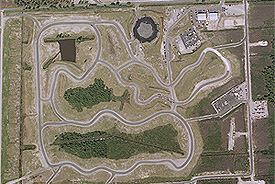
\includegraphics[width=\linewidth,keepaspectratio=true]{roundtrip/roundtrip}
\vspace{-9mm}
\end{wrapfigure}

\noindent
After The Stig's identity was revealed, the TV show Top Gear is in dire need of a new, tame racing driver to replace him. And of course you have been asked to take the job. However, you are not very fond of driving quickly, and especially not around the twisting and turning tracks they use in the show. To help you alleviate this problem, one of your algorithmic friends has suggested that you should calculate the roundtrip with the least possible amount of turning required. 

The driving track consists of unique, straight lines, and there are always exactly $2$ or $4$ roads heading out from each node. A roundtrip must be an Eulerian circuit, i.e. it must traverse each edge of the graph exactly once, and end up where it started. (Such a circuit is guaranteed to exist in the input graphs.) Thus the total amount of turning is the sum of the turning required at each node, where continuing in a straight line means a turn of $0$. The roads on the track can be driven in any direction.

\Input
One line with $3 \leq N \leq 10000$ -- the number of nodes -- and $N \leq M \leq 2N$ -- the number of edges.\\
$N$ lines with the $x$ and $y$ coordinates of each node, in order. $0 \leq x, y \leq 10000$. The nodes have unique coordinate pairs.\\
$M$ lines with two space separated numbers $i$ and $j$, denoting an edge between nodes $i$ and $j$. The nodes are $0$-indexed.\\

\Output
The least amount of turning you must do to complete an Eulerian circuit, in radians.\\

\Xample{roundtrip/roundtrip.1}

\Xample{roundtrip/roundtrip.2}

\begin{figure}
\centering
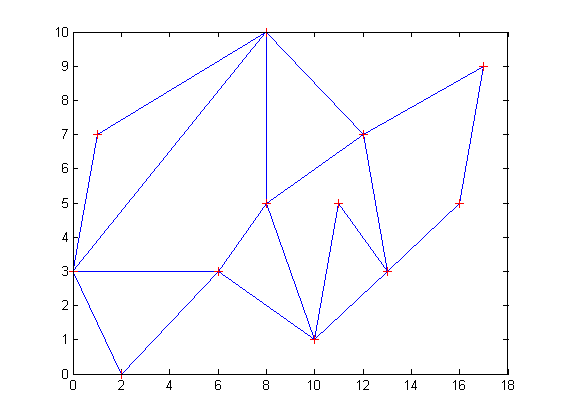
\includegraphics[width=\linewidth,height=150pt,keepaspectratio=true]{roundtrip/roundtrip2}
\caption{Figure of the second sample case}
\end{figure}